\documentclass[../dissertation.tex]{subfiles}
\begin{document}

\chapter{Implementation}
\label{chap:impl}

The Django Web App project contained 3 core components: 

\begin{itemize}
    \item The core Django app
    \item The Tulip Python API Wrapper, which controls all interactions between Django and Tulip
    \item The documentation app, which includes all of the front-end: the HTML/CSS, the interface, the Vis.js library and code, and the JavaScript library.
\end{itemize}

The core Django app included the URL paths for the whole project and the project settings, and no more.

\section{Tulip Python API Web Wrapper}

The web wrapper for the Tulip Python API was a major part of the project, and contained all interactions that Django had with Tulip. Tulip has a python package \cite{tulippip} that can be installed using pip \cite{pip}. Calls can then be made to the Python API from within Tulip, such as loading \texttt{.tlp}'s and running code against the loaded networks. The end result of this was enabling Tulip to be called by Django (after a user asked to visualise a network), and then creating a network in memory and running operations against it. 

Several critical design decisions had to be made throughout the creation of the web wrapper, listed below.

\subsection{Handling errors on the server}

A decision had to be made as to how the client would be made aware that the server had caught an error. Simply, there are three states which the server can return: success, expected error and unexpected error. From within Django there are many ways in which the errors can be dealt with. The page can simply be refreshed, flushing the error, a custom error page can be shown displaying the error code, such as 404, or an error can be passed back to the interface which can then be caught and displayed as appropriate. As one of the goals of the project was try to make the web wrapper a reusable API as opposed to a single use system, it was decided that each return would include a JSON object, which would include a success boolean, and then either the expected information (such as the network) or a message with why the error had occurred. It would then be down to the library that called the API to catch the JSON appropriately, and then the interface to act on them accordingly. For this application, it can be seen in Section \ref{sec:jslib} how the library and interface handled errors.

\subsection{Transferring networks to JavaScript}

There were two ways in which the network could be sent across a network to the user. These were:

\begin{itemize}
    \item Serialising the network and then recreating it from within JavaScript
    \item Transforming the network into JSON and then sending it over the network
\end{itemize}

The advantage of serialising and recreating the network fully in JavaScript is that the client then has access to the whole network and there is no data loss in the transaction. However, the advantage of transforming the network into JSON is both that the size of the transfer is less as only the required data needs to be sent (superfluous data can be cut out) and also that the client does not need to then recreate the network after receiving it (using computational power). Additionally, it would be possible to send the information over the network as a byte-array - which would be even more compact than JSON but sacrifice usability. 

It was decided that the data would be converted into JSON and then transferred over the network. This decision was made as high performance for massive networks was one of the main goals of the system, along with ensuring the system could easily be used by further developers. Transferring only what is necessary both reduces the amount of data that needs to be sent over the network, and also minimises the amount of processing required by the client. These are both ways to increase performance.

\subsection{Storing networks on the server}

Another critical design decision had to be made relating to how the networks were to be stored on the server. Upon further research, three possibilities presented themselves as to how this could be completed:

\begin{itemize}
    \item The structure of the network could be stored directly in a database's table. This could be done by having a table in the database for networks which would include a network ID, all of the nodes edges in a network.
    \item The \texttt{.tlp} of the network could be uploaded to the server and a link to that location could be saved in the database.
    \item The networks could all be saved on Hadoop's HDFS (explained in Appendix \ref{sec:whatishadoop}) so that working with Big Data would be supported.
\end{itemize}

The advantage of storing the network directly is that all data would be stored in a single database. For a small scale application, this would make managing the system easier and have no notable drawback. However, as many massive networks may be saved to the system, the database would quickly become very large and therefore its performance would suffer greatly. As a requirement for the system was that it would work on massive datasets, an alternative solution would have to be found. Out of the other two solutions, one involved saving all of the networks on the server, and the other on a HDFS cluster. 

The advantage of storing the networks on the server means that you can still store a massive amount of data on the server without the overhead and complications of setting up a Hadoop cluster. However, the advantage of using Hadoop is that it would allow for far more data to be stored in HDFS, and then MapReduce would allow for considerably faster processing of massive networks.

For this project, it was decided that the network would be stored on the server as this was a simpler approach that would be far quicker to get up and running, and additionally it would not be possible to acquire the resources needed to utilise Hadoop effectively.

This links in to another challenge faced - if a large amount of backing storage had been available to utilise then more experimentation could have been done into how the software interacts with massive amounts of data. However, as a result of not having this, the project was tailored in a way which meant that having large datasets was not required, and design decisions such as using Vis.js as opposed to D3.js were made, so differences in performance were more apparent.

\subsection{Bundling a network}

It had been decided that the three algorithms that were to be available to apply were Node Pruning, Node Bundling based on cliques and Node Bundling based on number of edges. Details of how these algorithms worked can be found below.

\subsubsection{Node Pruning}
\label{sec:impl-node-prun}

Node Pruning involves finding each node with only one edge and removing it from the network. Additionally, it is possible to include information about how many nodes have been bundled into each remaining node. This means less information is lost as a user can clearly see how many nodes with one edge were connected to each node that has been pruned. The algorithm for Node Pruning is outlined in Algorithm \ref{alg:node-pruning}.

\begin{algorithm}[H]
\caption{Defines the process for Node Pruning}
\label{alg:node-pruning}
\begin{algorithmic}
\STATE{G = (V,E)} \COMMENT{a graph containing vertices and edges}
\FORALL{V in G} 
    \IF{V has only 1 edge} 
        \STATE{add V to list to delete} 
    \ENDIF 
\ENDFOR
\FORALL{V in list to delete} 
    \STATE{delete V from G} 
\ENDFOR
\end{algorithmic}
\end{algorithm}

\subsubsection{Node Bundling based on cliques}
\label{sec:impl-node-clique}

This is calculated by using the \texttt{clusteringCoefficient} algorithm provided by Tulip \cite{tulip-clustering-coeff-doc}. Each node is assigned a value between 0 and 1, based on how close to a clique its neighbours are. For each node with a value near 1, an operation is done to bundle that node, shown below. It was decided that a \texttt{clusteringCoefficient} of greater than 0.8 was required for nodes to be bundled after several networks were tested against and less than that resulted in too much information being lost. The algorithm for Node Bundling based on cliques presented in Algorithm \ref{alg:node-bundling-clique}.

\begin{algorithm}[H]
\caption{Defines the process for Node Bundling based on cliques}
\label{alg:node-bundling-clique}
\begin{algorithmic}
\STATE{assign each node a clustering coefficient} \COMMENT{using Tulip's \texttt{tlp.clusteringCoefficient}}
\STATE{G = (V,E)} \COMMENT{a graph containing vertices and edges}
\STATE{initialise list toBundle}
\FORALL{V in G} 
    \IF{clustering coefficient of V is greater than 0.8}
        \STATE{add V to toBundle}
    \ENDIF
\ENDFOR
\FORALL{V in toBundle}
    \STATE{bundle V} \COMMENT{The code to bundle can be seen in Algorithm \ref{alg:bundle-node}} 
\ENDFOR

\end{algorithmic}
\end{algorithm}

\subsubsection{Node Bundling based on number of edges}

This is done by initially calculating the mean number of edges in the network. Then, any node that has greater than two times the mean number of edges is bundled, as explained below. Two times the mean was chosen after many sample networks were looked at based on data provided by SAS and this number seemed to be optimal in reducing the amount of data that needed to be passed to the client. Lowering the number resulted in too much data resulted in the visualisation loses meaning and increasing it meant there was little or no processing done in most cases. The algorithm for Node Bundling based on number of edges is outlined in Algorithm \ref{alg:node-bundline-edge}.

\begin{algorithm}[H]
\caption{Defines the process for Node Bundling based on number of edges}
\label{alg:node-bundline-edge}
\begin{algorithmic}
\STATE{G = (V,E)} \COMMENT{a graph containing vertices and edges}
\STATE{initialise integer edgeCounter}
\FORALL{V in G} 
    \STATE{add the degree of V to edgeCounter} 
\ENDFOR
\STATE{meanNumberOfEdges = edgeCounter/number of vertices in G}
\STATE{initialise list toBundle}
\FORALL{V in G} 
    \IF{degree of V greater than meanNumberOfEdges} 
        \STATE{add V to toBundle} 
    \ENDIF
\ENDFOR
\FORALL{V in toBundle} 
    \STATE{bundle the vertex with the highest degree} \COMMENT{The code to bundle can be seen in Algorithm \ref{alg:bundle-node}} 
\ENDFOR
\end{algorithmic}
\end{algorithm}

\subsubsection{Bundling a Node}

Upon discovering what nodes need to be bundled, the node then needs to be actually bundled. This involves locating all of the nodes neighbours, getting all of their edges, redirecting all of those edges to the node that is being bundled, and finally deleting each neighbour node. Algorithm \ref{alg:bundle-node} shows this process.

\begin{algorithm}[H]
\caption{Defines the process for bundling a node}
\label{alg:bundle-node}
\begin{algorithmic}
\STATE{aNode} \COMMENT{a node is passed in to this function to be bundled, aNode}
\STATE{initialise list neighbours}
\FORALL{neighbour of aNode} 
    \STATE{add neighbour to neighbours}
    \FORALL{edge of neighbour}
        \IF{edge not connected to aNode}
            \STATE{connect edge to aNode from neighbour}
        \ELSE
            \STATE{delete edge}
        \ENDIF
    \ENDFOR
\ENDFOR
\FORALL{node in neighbours}
    \STATE{delete node}
\ENDFOR
\end{algorithmic}
\end{algorithm}

\section{JavaScript Library}
\label{sec:jslib}

The JavaScript library involved creating a function to match each endpoint in the Tulip Python API Web Wrapper, which could be called from an interface. The main aim in creating the library was to make it as open and flexible as possible, allowing for developers to have access to exactly what they need, and on top of that be able to handle errors easily. Given that I had not developed a library before, research was done into the best way to take errors from the web wrapper and then pass them on to the interface. The outcome of this research was that the preferred way of error handling was to:

\begin{enumerate}
    \item Make the interface call a function with any parameters, a success callback, and an \emph{optional} error callback. An example of this can be seen in Listing \ref{listing:interf-to-jslib}
    
    \begin{lstlisting}[caption=How the interface would call the JavaScript library, label=listing:interf-to-jslib]
// graphToLoad = the name of the network to be loaded
tulipWebApi.loadGraph(graphToLoad, function(result) {
	networkCreator.drawSimpleGraph(result);
}, function(error) {
	console.error(error)
});
    \end{lstlisting}
    
    \item The library then receives the call and makes the appropriate AJAX call to the server, and upon getting a result it checks if the call was successful. Line 10 of Listing \ref{listing:jslib} shows this check
    \begin{enumerate}
        \item If the AJAX call was successful then the callback function passed in by the interface is called with the data requested, such as the network requested. This is shown on line 11 of Listing \ref{listing:jslib}.
        \item If the AJAX call failed then the library checks if an \texttt{errorCallback} function was passed in by the interface. If so, then that function is called and the error message is passed. If not, then nothing is called. This means that the library has the option of failing silently if the developer making the interface wishes. This is shown on lines 12 to 16 of Listing \ref{listing:jslib}.
    \end{enumerate}
    
    \begin{lstlisting}[caption=How the JavaScript library catches and passes errors, label=listing:jslib]
loadGraph: function(fileName, callback, errorCallback) {
	$.ajax({
		url: `/api/loadGraph',
		data: {
	        `network_name': fileName,
	    },
	    cache: false,
	    type: `GET',
		success: function(result) {
			if (result.success) {
        		callback(result.data);
			} else {
				if (typeof errorCallback === `function') {
					errorCallback(result.message);
				}
			}
        },
		error: function() {
			if (typeof errorCallback === `function') {
				errorCallback(`Unknown server error.');
			}
        }
    });
}
    \end{lstlisting}

\end{enumerate}

\section{Interface and Vis.js visualisation}
\label{sec:in-vis}

The interface involved catching events (such as button clicks) and then calling the appropriate JavaScript library function. If the call is successful then a success message appears and/or an action is executed, and if not then an error is outputted to the console and potentially to the DOM. 

One of the core actions the front end was required to do is to actually render a network. This was done by taking in all the information passed to it by the JavaScript library, then converting all of the nodes and edges into two arrays, along with stylising them appropriately based on if they had been bundled or pruned, and then initialising the network. This involved specifying the container where the network would be rendered, the data it would contain and any optional parameters. A summary of this can be seen in Listing \ref{listing:vis-js}.

\begin{lstlisting}[caption=How to create a network using Vis.js, label=listing:vis-js]
drawSimpleGraph: function(result) {

    arrayOfNodes = [];
    arrayOfEdges = [];
    
    for (var i = 0; i < result.nodes.length; i++) {
        arrayOfNodes.push({id: i, label: i});
        result.nodes[i].outEdges.forEach(function(element) {
            arrayOfEdges.push({from: i, to: element})
        });
    }
    
    var nodes = new vis.DataSet(arrayOfNodes);
    var edges = new vis.DataSet(arrayOfEdges);
    
    var container = document.getElementById(`main_network');
    
    // provide the data in the required vis.js format
    var data = {
        nodes: nodes,
        edges: edges
    };
    
    var options = { /* Setting many layout and physics parameters */ }
    
    // initialise the network
    var network = new vis.Network(container, data, options);
}
\end{lstlisting}

There are several different variables that can be set in \texttt{options} on line 24 of Listing \ref{listing:vis-js}. A full list of options can be seen on the Vis.js website \cite{visjsoptions}. Several options were experimented with for this project, details of which can be seen below. 

\subsection{Layout}

Within the \texttt{layout} \cite{visjslayout} option, if \texttt{improvedLayout} was set to \texttt{false}, then Kamada Kawai Algorithm \cite{kamada1989algorithm} is \emph{not} applied, which reduces stability of the network but improved rendering times. This parameter was toggled multiple times throughout testing and was found to rarely be beneficial to the visualisation as a whole when disabled, despite decreased rendering times. Thus, it was decided to set it to \texttt{true} for this system.

\subsection{Physics}

In the \texttt{physics} \cite{visjsphysics} option, there were several different parameters which could be finely tuned. The first of these was \texttt{stabilisation}, which selected if the network should be stabilised or not, and if so, by what means. It was decided that it would be enabled, as disabling it caused the network to move too erratically on load - despite loading far sooner. 

Additionally, the maximum and minimum speed could be set, the time between steps could be changed, and the model for the physics solver could be selected. This could be one of four preset solvers: \texttt{barnesHut} \cite{barnes1986hierarchical}, \texttt{forceAtlas2Based} (based on the Force Atlas 2 algorithm \cite{jacomy2014forceatlas2}), \texttt{hierarchicalRepulsion}, or \texttt{repulsion}. Alternatively, a custom model could be supplied. A custom solver could take in the following arguments: \texttt{gravitationalConstant}, \texttt{centralGravity}, \texttt{springLength}, \texttt{springConstant}, \texttt{damping} and \texttt{avoidOverlap}. Although time was spent exploring the physics module and creating several custom solvers, the custom solvers tended to perform more poorly than the preset solvers, and the default option worked the best in most scenarios. 

Additionally, it was possible to disable the Physics module entirely and the network would be displayed in a ring, with nodes equally spaced and edges placed appropriately. This lead to near instant loading times but the visualisations becoming meaningless, so the module remained enabled.

\subsection{Nodes}

The \texttt{nodes} option allowed for each node to be customised. Options included the nodes: size, colour, shape, font, label, border and mass. These could be set for all nodes in the network or individually - and these options were used extensively to illustrate to a user what nodes had been bundled how much bundling had occurred.

\subsection{Interaction}

It was also possible to edit how users could interact with the visualisation through the \texttt{interaction} option. This allowed for: users to select multiple nodes, nodes to be locked into place or free for the user to move, nodes to show tooltips which could contain additional information, and the ability to zoom in or out. Zooming on the network and interaction with nodes was enabled so users could get more detailed information on the network and how it reacted to different nodes being moved. Future iterations of the project could include using tooltips to give more information about each node, depending on what was being visualised.

\section{Front-end}

\subsection{Architecture}

The front-end of the system was written using HTML, CSS and JavaScript. The HTML was written in Django Templates \cite{django-docs-templates}, and a base file was written which acted as a container for each of the other HTML files. A CSS framework, Bootstrap \cite{bootstrap} was utilised in order to allow for a smart interface to be created very quickly, and ensure that development time was not spent on creating a user interface from scratch. The JavaScript for the system used jQuery \cite{jQuery}, which made interacting with the DOM a very easy process. JavaScript was user to pick up events based on user interactions and make appropriate calls to the JavaScript library detailed in Section \ref{sec:jslib}.

\subsection{System Interaction}

To use the finished system, a user would simply select a network to visualise, decide which algorithms would be applied to the network using check boxes, and then select `Load'. This can be seen in Figure \ref{fig:topbar}.

\begin{figure}[H]
    \centering
    
\includegraphics[width=15cm]{7/topbar}
    \caption{This shows how a user would interact with the system to view a network}
    \label{fig:topbar}
\end{figure}

The two other key components of the front-end were uploading and deleting networks. Uploading a network involved: naming the network and selecting either a \texttt{.tlp} or a \texttt{.json} (in SAS's format) file. A \texttt{.tlp} could be loaded directly into the system and would be saved directly. However, the \texttt{.json} file would have to be converted to a \texttt{.tlp} so Tulip could understand it. This involved uploading the \texttt{.json} file, creating a \texttt{.tlp} file the same name but a different file extension, parsing the \texttt{.json} file, and then copying the relevant information into the blank \texttt{.tlp} file. Deleting a network was done by selecting the network to be deleted from a drop-down list, and clicking `Delete'.

\subsection{Finished Product Screenshots}

Figure \ref{fig:1000-none} and \ref{fig:1000-both} show the final product rendering a network of 1000 nodes, and then rendering the same network after it had been Node Pruned and Node Bundled based on number of edges. These both show how Vis.js visualise networks and what the system looks like, and also show the benefit of processing networks on the server. Figure \ref{fig:1000-none} took 59924ms to load and Figure \ref{fig:1000-both} took 153ms to load, further highlighting the benefits of the system.

\begin{figure}[H]
    \centering
    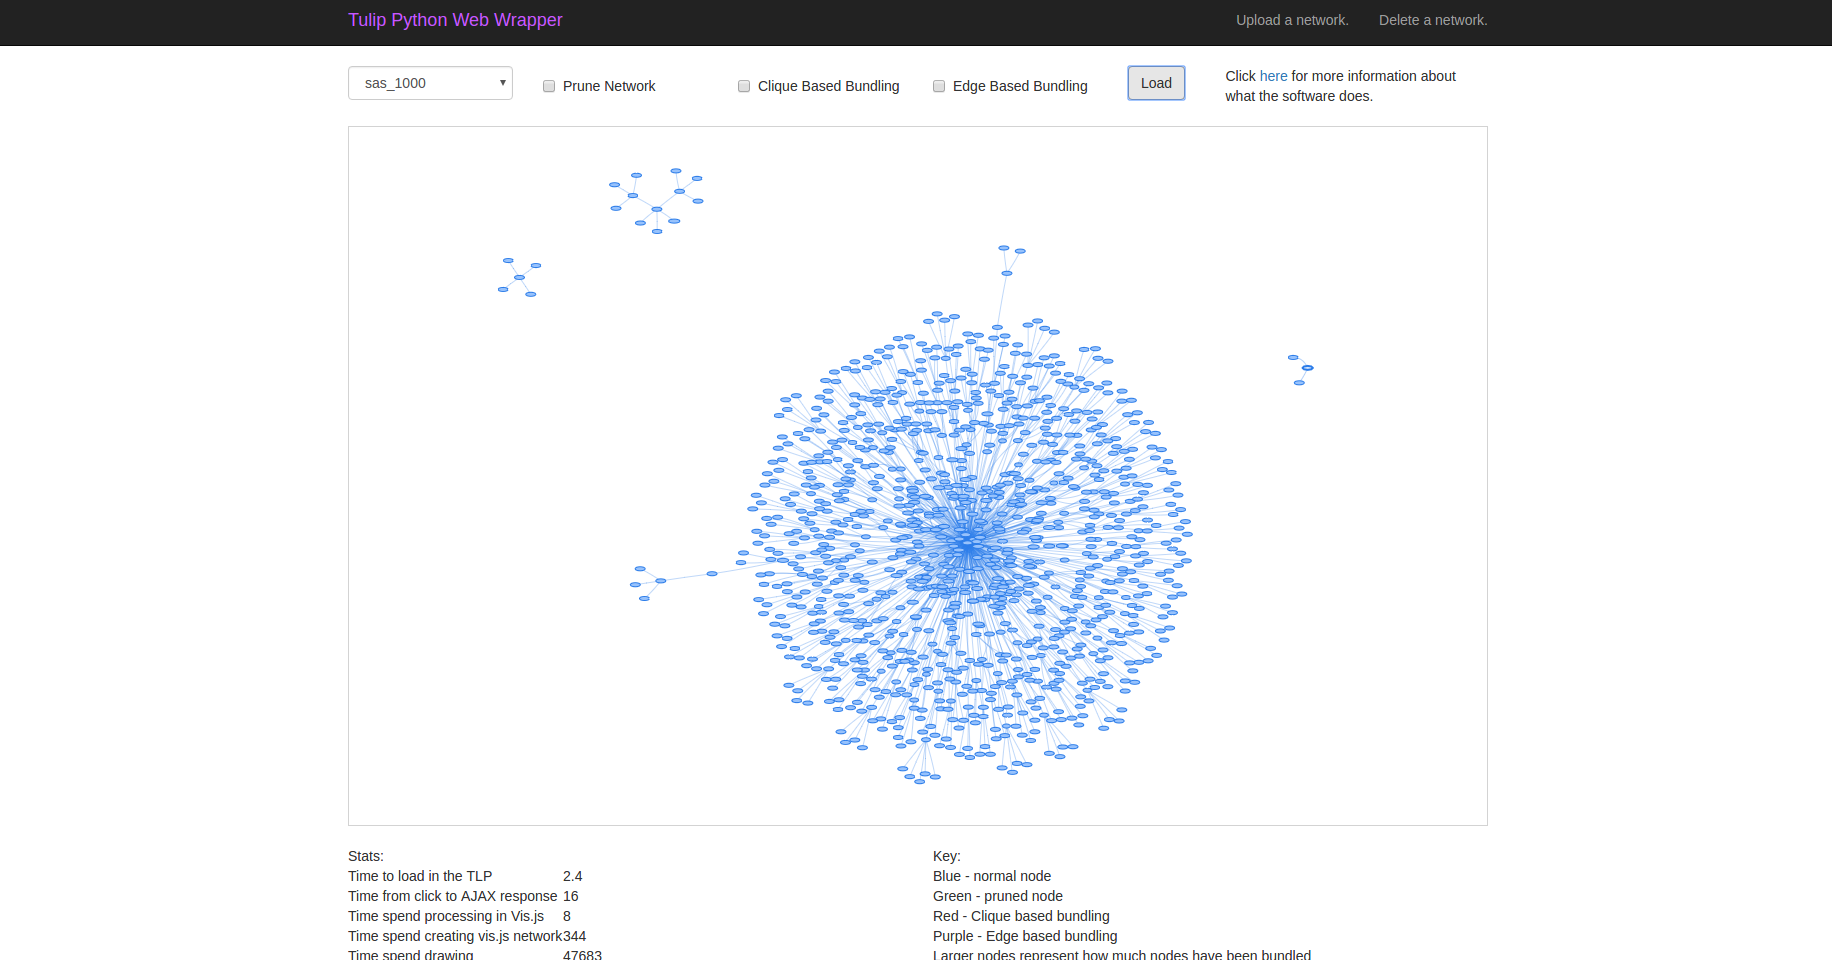
\includegraphics[width=15cm]{7/1000_1none}
    \caption{This shows the system visualising a network with 1000 nodes without any processing taking place.}
    \label{fig:1000-none}
\end{figure}

\begin{figure}[H]
    \centering
    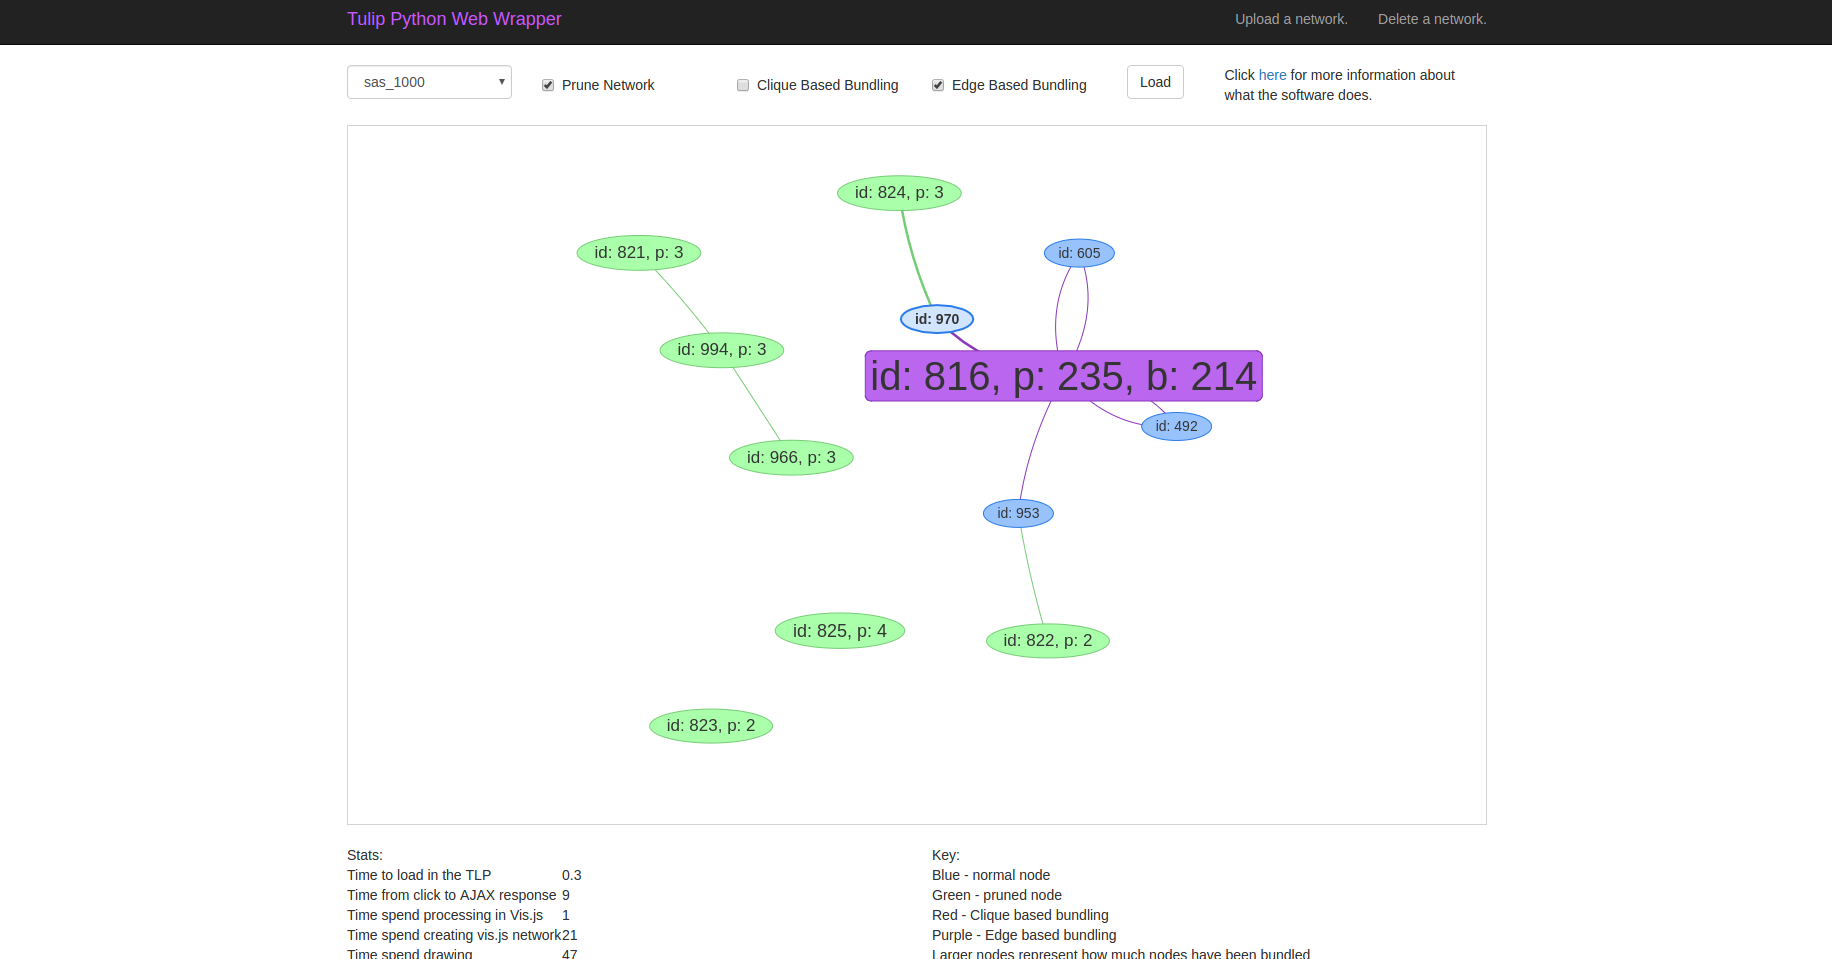
\includegraphics[width=15cm]{7/1000_4both}
    \caption{This shows the same network as seen in Figure \ref{fig:1000-none}, but with Node Pruning and then Node Bundling based on number of edges applied to it.}
    \label{fig:1000-both}
\end{figure}

\end{document}